\documentclass{standalone}
\usepackage{standalone}

\begin{document}
\section{Segmentation}
The goal of this stage is to separate all characters into different image to send them to OCR for recognition. We used horizontal and vertical projections in this step.


\subsection{Horizontal Segmentation}
Horizontal projection is done my taking mean of all columns across the rows of the image. Figure \ref{fig:HorizontalProjection} shows a graph of mean values across the rows. To calculate this mean we followed the formula from Algorithm \ref{eq:HorizontalProjection}. We set the cutoff line to be $\geq 1$. and separated the entire plate into two segments. 

\begin{algorithm}
  \begin{algorithmic}
    \For{\texttt{i:=1 to height}}
        \State $P_i = \dfrac{ \sum^{width}_{i=1}{ I_{ij} } }{ width }$
    \EndFor
  \end{algorithmic}
  \caption{Horizontal projection algorithm}
  \label{eq:HorizontalProjection}
\end{algorithm}

\begin{figure}
\centering
\begin{subfigure}{0.8\textwidth}
  \centering
  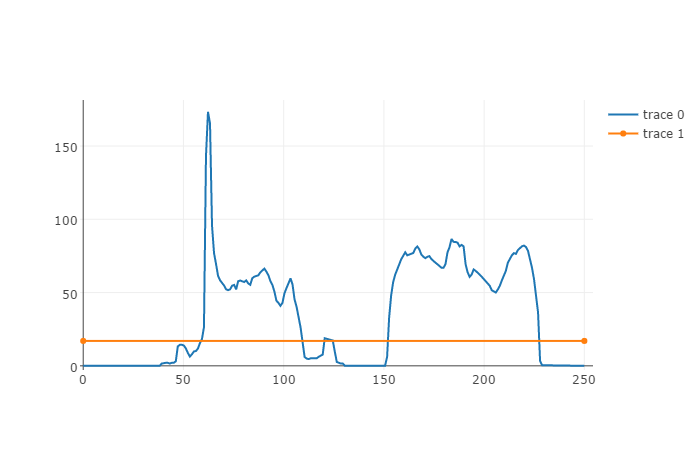
\includegraphics[width=0.8\linewidth]{./img/plots/horizontal-1}
  \caption{Horizontal projection plot}
\end{subfigure}
\begin{subfigure}{0.8\textwidth}
  \centering
  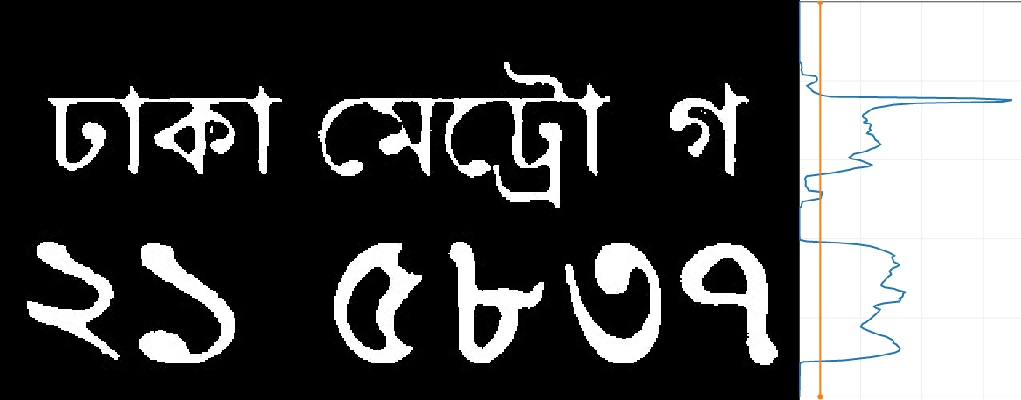
\includegraphics[width=0.8\linewidth]{./img/plots/horizontal-2}
  \caption{Comparing the image against its projection}
\end{subfigure}
\caption{Horizontal projection of plate image.}
\label{fig:HorizontalProjection}
\end{figure}



\subsection{Vertical Segmentation}
We calculated the vertical projection using similar algorithm (Algorithm \ref{eq:VerticalProjection}). The result of the projection is shown in Figure \ref{fig:VerticalProjection}.

\begin{algorithm}
  \begin{algorithmic}
    \For{\texttt{j:=1 to width}}
        \State $P_j = \dfrac{ \sum^{height}_{i=1}{ I_{ij} } }{ height }$
    \EndFor
  \end{algorithmic}
  \caption{Vertical projection algorithm}
  \label{eq:VerticalProjection}
\end{algorithm}

\begin{figure}
\centering
\begin{subfigure}{0.8\textwidth}
  \centering
  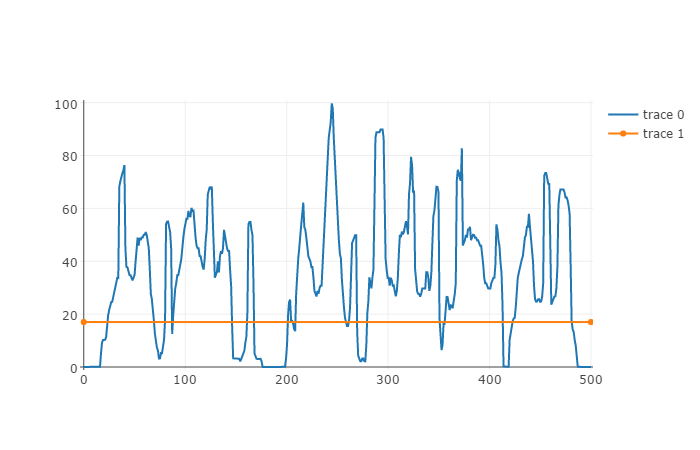
\includegraphics[width=0.8\linewidth]{./img/plots/vertical-1}
  \caption{Vertical projection plot}
\end{subfigure}
\begin{subfigure}{0.8\textwidth}
  \centering
  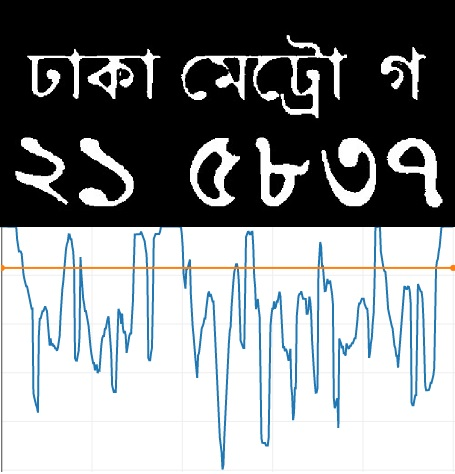
\includegraphics[width=0.8\linewidth]{./img/plots/vertical-2}
  \caption{Comparing the image against its projection}
\end{subfigure}
\caption{Vertical projection of plate image.}
\label{fig:VerticalProjection}
\end{figure}


\end{document}